\Tr
\onecolumn
{\red
\begin{center}
Exercise
\end{center}
\begin{itemize}
\item Consider very nearby objects such that the observed redshift $z$ can be interpreted
      as a Doppler shift due to the recession velocity $v$ of the object.
\item[$\ast$] Derive that the distance $r$ of the object can be determined as
              $r=\frac{c}{H_{0}} \cdot \frac{(1+z)^{2}-1}{(1+z)^{2}+1}$
\item For some relatively nearby Gamma Ray Bursts (GRBs) the fluence $S$ in gamma rays and $z$
      have been measured by the Batse and BeppoSax satellites.
      Assuming isotropic emission over the full solid angle, all these bursts seem to have
      more or less the same energy output $E_{0}$ of about $10^{52}$ erg.
\item[$\ast$] Assume a characteristic isotropic energy output of $E_{0}$ for all GRBs and a
              homogeneous GRB number density $n$. Neglect redshift effects.\\
              Show how $n$ can be determined by only a measurement of the fluence of the various bursts.\\
              {\black Hint : Investigate the cumulative GRB count above a certain reference fluence}
\item In the plot below the cumulative GRB count $N(>S)$ of GRBs with a fluence exceeding a certain reference fluence $S$
      is presented as a function of this reference fluence $S$.\\
      It is seen that at high $S$ the plot approaches a straight line with a slope of about -1.5.
%
\newpage
%
\item[$\ast$] Explain the linear behaviour and slope value at high $S$.
\item[$\ast$] Give a possible explanation for the flattening at lower $S$ values.
\item[$\ast$] What could be a reason for the saturation effect at the lowest $S$ values ?
\end{itemize}
}%%% End of red area
%
\begin{center}
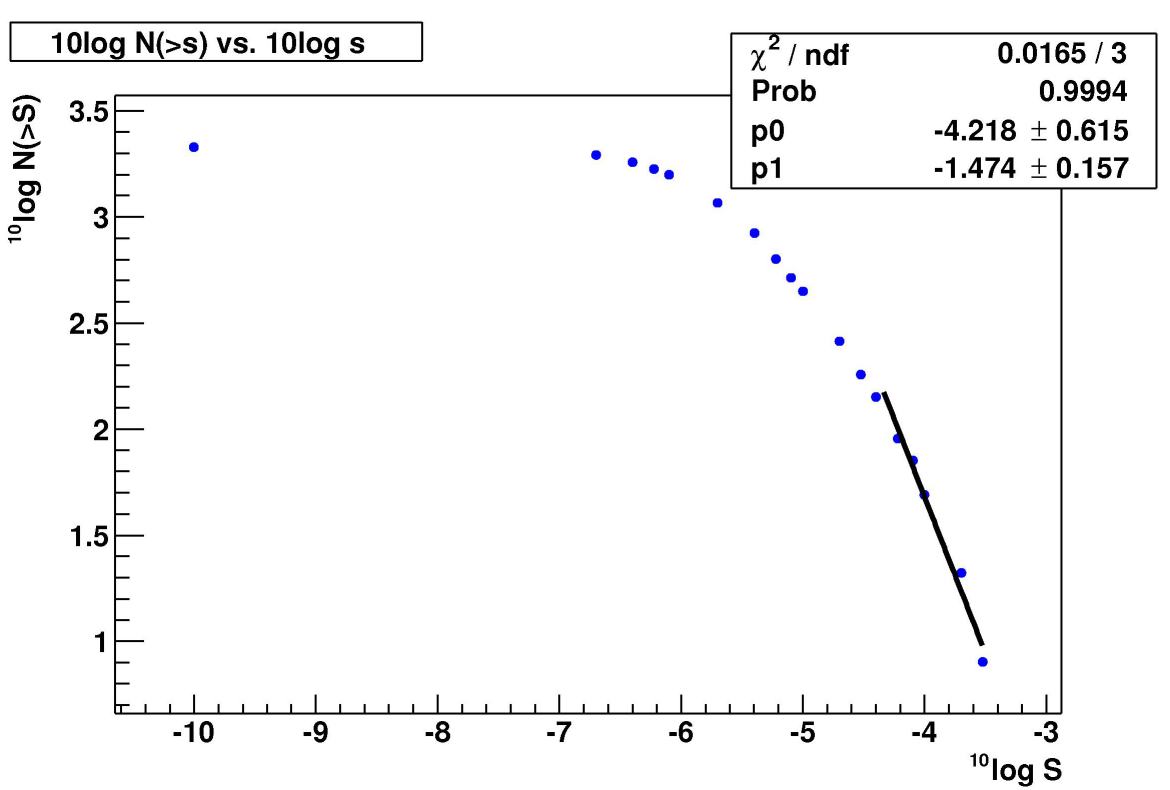
\includegraphics[keepaspectratio,width=15cm]{batse-n-s}
\end{center}

\Tr
\onecolumn
\begin{center}
\colorbox{yellow}{Using the NcAstrolab facility of NCFS-Pack}
\end{center}
%
\begin{itemize}
\item At the {\blue IIHE} everything has been centrally pre-installed in {\blue NCFS-Pack}
\item[] Login to the central IIHE computer portal as indicated at the lectures
\item[] For once issue the command {\blue \tt cp /ice3/software/iihe/.rootrc \$HOME}
\item[] At the command prompt enter {\blue \tt source /ice3/software/iihe/ncfs.sh}
\item[] This initialises the package and sets the prompt to {\blue \tt ncfs$>$} 
{\red
\item[$\ast$] Now you are able to use the ROOT framework
}
\item[] ROOT session : at the command prompt {\blue \tt ncfs$>$} just type {\blue \tt root}
\item[] Running a ROOT macro : {\blue \tt ncfs$>$ root -b -q test.cc $>$test.log}
\item \colorbox{yellow}{Loading NCFS-Pack into a ROOT session or macro}
\item[] {\blue \tt gSystem->Load("ncfspack");}
\item Online ROOT docs are available via http://root.cern.ch
\item Online NCFS-Pack docs are available via https://nick-ve.github.io/ncfs/docs
\end{itemize}

\Tr
\onecolumn
\begin{center}
\colorbox{yellow}{The NcAstrolab facility}
\end{center}
%
\begin{itemize}
\item {\blue NcCollider} provides a tool to {\blue simulate various high-energy collision processes} 
\item {\blue NcAstrolab} provides a virtual laboratory to {\blue analyse (astro)physical phemomena}
\item[] It contains various analysis tools like :
\begin{itemize}
\item Conversion between various (astrophysical) coordinate systems
\item Various date and time systems (e.g. Julian dates and siderial times)
\item Determination of nuclear masses and binding energies
\item Determination of distances on cosmological scales
\item Matching of lab. observations with astrophysical objects and skymap displays
\end{itemize}
\end{itemize}
%
{\red
\begin{center}
Exercise
\end{center}
%
\begin{itemize}
\item Consider a flat Friedmann-LeMa\^{i}tre universe.
\item Use the NcAstrolab facility to produce a plot with on the X-axis the redshift $z$
\item[] and on the Y-axis the physical distance $D(z)$ for objects with $0<z<15$.
\end{itemize}
}%%% End of Red area

\Tr
{\red
\begin{center}
Analysis of the NASA Swift satellite GRB data
\end{center}
%
\begin{itemize}
\item GRB data of the NASA Swift satellite are available at
\item[] http://swift.gsfc.nasa.gov/docs/swift/archive/grb\_table
\item Assume that GRBs emit their energy isotropically over the full $4\pi$ solid angle
\item[$\ast$] Investigate whether every GRB emits about the same amount of energy
\item Assume that GRBs emit their energy in 2 back to back jets with a jet cone of $3^{\circ}$
\item[$\ast$] What will be the difference w.r.t. the previous analysis ?
\item[$\ast$] What would this imply for the GRB rate in the Universe ?
\end{itemize}
}%%% End of Red area
